%!TEX root = thesis.tex

\chapter{Monitoring Timing Constraints on possibly infinite Streams}
\label{chapter-monitorability}
	The goal of this thesis is to implement online monitors for the TADL2 Timing Constraints on possibly infinite streams. An online monitor checks the current execution of a system, parallel to its execution. Because every computing system has finite memory resources and the online monitor should be able to process at least as many events as occur in the stream in a specific amount of time, not every property can be monitored in an online monitoring setting. In this chapter, the term of \emph{Simple Monitorability} will be introduced, which ensures that monitoring a property on infinite streams is possible with finite memory resources and finite run time per event. As introduction into the setting, some related work will be described, inter alia \emph{TeSSLa}, the programming language which is used for the implementation.

\section{Related Work}

	\subsubsection{Runtime Verification}
		As monitoring plays a major role in runtime verification, a short overview of this will be given. The definitions of \cite{RuntimeVerification} are used, in which \emph{Runtime Verification} is a technique that can detect deviations between the run of a system and its formal specification by checking correctness properties. A \emph{run}, which might also be called \emph{trace}, is a sequence of system states, which might be infinite and an \emph{execution} is an finite prefix of this run. A \emph{monitor} reads the trace and decides, whether it fulfills the correctness properties or violates them.\\
		A distinction is made between \emph{offline} and \emph{online} monitoring. Offline monitoring is using a stored trace, that has been recorded before. Therefore, the complete trace (or the complete part of the trace, that should be analyzed) is known in the analysis. Online monitoring checks the properties, while the system is running, which means that the analysis must be done incrementally on a growing prefix of the trace. Because of memory and time limitations, not all previous states can be read again in online monitoring, more detailed contemplations on the limitations of online monitors will be given in in this chapter.

	\subsubsection{TeSSLa}
		TeSSLa (\textbf{Te}mporal \textbf{S}tream-based \textbf{S}pecification \textbf{La}nguage) \cite{TeSSLa1} is a specification language build for Stream Runtime Verification. In TeSSLa, all streams in one specification must have a common global clock, but events or changes in a signal may occur in streams irregularly, independent of events in other streams. The verified streams are either considered as signal, which remain unchanged for a certain amount of time (called \textit{piece wise constant signals}), or they are \textit{event streams}, in which each event consists of a timestamp and a data value. Both variants can be transferred into each other, like described in \cite{TeSSLa1}. A formal definition of the TeSSLa language core can be found in \cite{TeSSLa2}, a short overview of the formal definition of event streams will be given next.\\
		An event stream is defined over a time domain $\mathbb{T}$ and a data domain $\mathbb{D}$ and is a possibly infinite sequence $s=a_0a_1...\in\mathcal{S}_D=(\mathbb{T}\cdot\mathbb{D})^\omega\cup(\mathbb{T}\cdot\mathbb{D})^+\cup(\mathbb{T}\cdot\mathbb{D})^*\cdot(\mathbb{T}_\infty\cup\mathbb{T}\cdot\{\bot\})$ where $a_{2i} < a_{2(i+1)}$ for all $i$ with $0 < 2(i + 1) < |s|$ ($0 < 2(i + 1) < \infty$ if the sequence is infinite). While the data domain $\mathbb{D}$ can be bounded (e.g. boolean or integer) or unbounded (e.g. maps or lists), the time domain $\mathbb{T}$ is a \emph{totally ordered semi-ring} $(\mathbb{T}, 0, 1, +, *, \leq)$ that is not negative.\\
		In TeSSLa, computations are done in timestamps, in which new events are arriving. Based on the specification, output streams are generated with events on the same timestamps as the used input streams, but filtering is possible, where not all input events produce output events. With the \textit{delay}-operator, it is possible to create new timestamps. If the \textit{delay}-operator is not used in a specification, the output streams only contains events in timestamps, which also had events in the input streams. These specifications are called \textit{timestamp conservative}.\\
		In a memory perspective, streams may be understood as \textit{piece wise constant signals}. Only the timestamp and the data value of the youngest event of one stream can be directly accessed. This event is available until the next event of this stream occurs. With the use of the \textit{last}-operator, which can be used recursively, the data value of the previous event can be accessed. Another important operator is the \textit{lift}-operator, which applies a function on data values (for example the $+$ operator) on the data value of every event of one or more streams and creates a new stream with events at the same timestamps and the results of the function as data values.
		
	\subsubsection{LOLA}
		\cite{LOLA} introduces \textit{LOLA}, a specification language for the observation of synchronous event streams, comparable to TeSSLa. The main difference between these languages is, that TeSSLa is designed to monitor input streams, which are not synchronized, which means their events may occur independently from each other. Because the events of the timing constraints defined in TADL2 and AUTOSAR are also not synchronized, TeSSLa is more suitable for monitoring them.\\
		\cite{LOLA} also defines the term of \textit{Efficiently Monitorable Specifications}, which describes that the worst case memory requirement of a LOLA Specification is independent of the length of the observed trace.
	
	\subsection{Transducer Models}
		In section~\ref{sec:monitorability}, some transducer models are used, which will be introduced next.
		\begin{definition}[Deterministic Finite State Transducer\cite{Berstel1979}]
			A \textit{Deterministic Finite State Transducer}(DFST) is a 5-Tuple $(\Sigma, \Gamma, Q, q_0, \delta)$, where
			\begin{itemize}
				\item
				$\Sigma$ is an input alphabet
				\item
				$\Gamma$ is an output alphabet
				\item
				$Q$ is a finite set of states, with initial state $q_0$
				\item
				$\delta:Q\times\Sigma\rightarrow Q\times\Gamma$ is a state transition function 
			\end{itemize}
			The run of a DFST for an input word $w=w_0w_1w_2...\in\Sigma^\infty$ is a sequence $s_0\xrightarrow{w_0/o_0} s_1\xrightarrow{w_1/o_1} s_2...$, where $s_0=q_0$, $\delta(s_i,w_i)=(s_{i+1}, o_i), i \geq 0$ and the output word $o=o_0o_1o_2...\in\Gamma^\infty$.
		\end{definition}
		DFSTs are similar to deterministic finite automata, with two major differences. First, the transition function outputs a symbol of $\Gamma$ at every transition and second, the states of a DFST are not accepting. The transducer \textit{transduces} an input word, not accepting or rejecting it.\\ \\
		Timed Deterministic Finite State Transducer(TDFST) are an extension of DFST. The extension from DFST to TDFST is done analogous to the extension of automata to timed automata in \cite{ALUR1994183}.
		\begin{definition}[Timed Deterministic Finite State Transducer]
			\textit{Timed Deterministic Finite State Transducers}(TDFST) are a 6-Tuple $(\Sigma, \Gamma, Q, q_0, C, \delta)$, where
			\begin{itemize}
				\item
				$\Sigma$ is an input alphabet
				\item
				$\Gamma$ is an output alphabet
				\item
				$Q$ is a finite set of states, with initial state $q_0$
				\item
				$C$ is a set of clocks
				\item
				$\delta:Q\times\Sigma\times\Theta(C)\rightarrow Q\times 2^C\times\Gamma$ is a state transition function, where for all $(q_a, \sigma_a, \vartheta_a, q_a', R_a, \gamma_a), (q_b, \sigma_b, \vartheta_b, q_b', R_b, \gamma_b)\in \delta$ the conjunction $\vartheta_a\land\vartheta_b$ is unsatisfiable. 
			\end{itemize}
			Let $v_i:C\rightarrow R$ be functions that map each clock to its current value.
			
			The run of a TDFST for an input word $w=(w_0,t_0)(w_1,t_1)(w_2,t_2)..., w_i\in\Sigma^\infty$ is a sequence $s_0, v_0\xrightarrow[o_0]{(w_0, t_0),\vartheta_0,r_0}s_1,v_1\xrightarrow[o_1]{(w_1, t_1),\vartheta_1,r_1}s_2,...$ with output $o=o_0o_1o_2...\in \Gamma^\infty$, if, and only if, 
			\begin{itemize}
				\item
					$s_0=q_0$
				\item
					$\forall c\in C: v_0(c)=0$
				\item
					$\forall i\geq 0:$
					\begin{itemize}
						\item
							$\delta(s_i, w_i,\vartheta_i)=(s_{i+1},r_i,o_i)$
						\item
							$\forall c\in r_i: v_{i+1}=v_i[c\leftarrow t_i]$
						\item
							$t_i,v_i \models\vartheta_i$
					\end{itemize}
			\end{itemize}
		\end{definition}
		In addition to DFSTs, the state transition function of TDFSTs takes a set of clock constraints into account when defining the next state of the transducer.
	
\section{Monitorability}
	\label{sec:monitorability}
	In this section, the term \textit{Simple Monitorability} is introduced. It represents a stricter alternative to \textit{Efficiently Monitorable Specifications} mentioned above, by also restricting the allowed run time per timestamp with events. \textit{Simple Monitorability} ensures, that the worst case memory consumption and the worst case run time per input event of a monitor is bounded independently of the input streams. 
	\subsubsection{Preliminary - Timestamps}
		\label{monitorability_timestamps}
		As we consider possibly infinite streams, the time value of events can also grow into infinity. This is problematic, because it leads to infinite memory requirements, which cannot be met, especially not in the context of online monitoring. Therefore, the time domain $\mathbb{T}$ is restricted by the following constraints:
		\begin{enumerate}[1.]
			\item
				The first used timestamp has the value $t_0=0$
			\item
				All used timestamps must be smaller than $t_{max}$.\\
				$t_{max}$ must be big enough, so it is not reached in practical use \footnote{for example, a 64-bit unsigned integer variable is enough, to cover nanoseconds for 584.55 years}.
			\item
				The distance between two subsequent time values is predetermined, but arbitrary small.
			\item
				The number of possible timestamps is significantly larger than the number of events.
		\end{enumerate}
	Because of the 2., 3. and 4., a limitation of the number of events in a specific time interval through these restrictions is invalid.

	\subsection{Simple Monitorability}
		The concept behind the definition of \textit{Simple Monitorability} is that a monitor for event streams is defined by three parts, a state transition function, a state defining the memory of the monitor and an output function. At each timestamp containing input events, the new state is created by applying the state transition function to the previous state and the input events of the current timestamp. The output function is applied to the new state and the previous output and evaluates, whether the specification is met until this timestamp.\\
		All following definitions of streams and functions follow the syntax and semantic from \cite{TeSSLa2}. The left half of figure~\ref{fig:OverviewMonitorability} visualizes the definitions, which will be done now.
		\begin{definition}[Simple Monitorability]
			A property is called \textit{Simple Monitorable}, if a monitor, which outputs $true_{until}$, as long as the property is fulfilled and $false$ after that, can be constructed in the following way:
			\begin{itemize}
				\item[\textbf{Input Streams}]
					Let $S_1, S_2, ..., S_n$ be the input streams with\\
					$\forall i:$ $S_i=(\mathbb{T}\cdot \mathbb{D}_i)^\omega\cup(\mathbb{T}\cdot \mathbb{D}_i)^+\cup(\mathbb{T}\cdot \mathbb{D}_i)^*\cdot(\mathbb{T}_\infty\cup\mathbb{T}\cdot\{\bot\})$
				\item[\textbf{State}]
					Let $S_{state}$ with $S_{state}= (\mathbb{T}\cdot \mathbb{D}_{state})^+\cup(\mathbb{T}\cdot \mathbb{D}_{state})^*$ be the state stream of the monitor. The cardinality of $\mathbb{D}_{state}$ is finite and the worst case memory requirement is bounded independently of the input streams.\\
					Further let $f: S_1 \times S_2 \times ... \times S_n \times S_{state}\rightarrow S_{state}$ be a state transition function, which defines the state stream in an incremental fashion:\\
					\begin{math}
						\forall t\in \mathbb T \exists i\in \{1,2,...,n\}: S_i(t)\in\mathbb D_i:\\
						S_{state}(t)= f(S_1(t), S_2(t), ..., S_n(t), last(S_{state}, merge(S_1, S_2, ..., S_n))(t))
					\end{math}\\
					The worst case run time of $f$ is bounded independently of the input streams.
				\item[\textbf{Output Stream}]
					Let $S_{output}= (\mathbb{T}\cdot \{true_{until}, false\})^+\cup(\mathbb{T}\cdot \{true_{until}, false\})^*$\\
					be the output stream of the monitor, which is defined via a function\\
					$g:S_{state}\times S_{output}\rightarrow S_{output}$\\
					which defines the output stream in an incremental fashion:\\
					\begin{math}
						\forall t\in \mathbb T \exists S_{state}(t)\in\mathbb D_i:\\
						S_{output}(t)= g(S_{state}(t), last(S_{output}, S_{state})(t))
					\end{math}\\
					The worst case run time of $g$ is bounded independently of the input streams.
			\end{itemize}
		\end{definition}
		In every timestamp with input events, the state transition function $f$ is applied to the current youngest input events and the previous event of the state stream $S_{state}$. The output of $f$, combined of the timestamp of the latest input event, defines the new event in $S_{state}$. The output of function $g$ is applied to the current state and the previous output and produces the new output. It should be noted that a monitor, which follows this scheme is \textit{timestamp conservative}.\\
		For any monitor, which is created in the way described above, a Deterministic Finite State Transducer (DFST) can be constructed, which is equivalent to the combination of a finite state and the state transition function. For that, let
		\begin{itemize}
			\item
			$Q=\mathbb{D}_{state}$ be the finite set of possible states with initial state $q_0$
			\item
			$\Sigma=((\mathbb{D}_1\times \mathbb{T}),...,(\mathbb{D}_n\times \mathbb{T}))$ be the input alphabet
			\item
			$\Gamma = \mathbb D_{state}$ be the output alphabet and
			\item
			$\delta: Q\times \Sigma\rightarrow Q\times\Gamma$ be the transition function.
		\end{itemize}
		For the output stream in combination with the output function, an equivalent DFST can be constructed too. For that, let
		\begin{itemize}
			\item
				$Q' = \{true_{until}, false\}$ be the states with initial state $true_{until}$
			\item
				$\Sigma'=\mathbb D_{state}\times \mathbb{T}$ be the input alphabet
			\item
				$\Gamma' = \{true_{until}, false\}$ be the output alphabet and
			\item
				$\delta': Q'\times \Sigma'\rightarrow Q'\times\Gamma'$ be the transition function.
		\end{itemize}
		It should be noted, that both transducers could be combined into one transducer without changing the expressiveness. This is not done to keep analogies to the following definition.
	\subsection{Simple Monitorability With Delay}
		Most of the TADL2 constraints can not be monitored correctly in a \emph{timestamp conservative} way. For example, the \emph{RepeatConstraint} with the attributes $lower=upper=4$ and $span=1$ expects subsequent events to have a time distance of $4$. If one event is missing, the output of a timestamp conservative monitor would remain $true_{until}$, until the next input event arrives. Therefore, the monitor cannot not check the constraint correctly. Because of this problem, the definition of \emph{Simple Monitorability} is expanded by the ability of introducing exactly one new timestamps. The following definitions are visualized in the right half of figure~\ref{fig:OverviewMonitorability}.
	\begin{definition}[Simple Monitorability With Delay]
		A property is called \textit{Simple Monitorable With Delay}, if a monitor, which outputs $true_{until}$, as long as the property is fulfilled and $false$ after that, can be constructed in the following way:
		\begin{itemize}
			\item[\textbf{Input Streams}]
				Let $S_1, S_2, ..., S_n$ be the input streams with\\
				$\forall i:$ $S_i=(\mathbb{T}\cdot \mathbb{D}_i)^\omega\cup(\mathbb{T}\cdot \mathbb{D}_i)^+\cup(\mathbb{T}\cdot \mathbb{D}_i)^*\cdot(\mathbb{T}_\infty\cup\mathbb{T}\cdot\{\bot\})$
			\item[\textbf{State}]
				Let $S_{state}$ with $S_{state}= (\mathbb{T}\cdot \mathbb{D}_{state})^+\cup(\mathbb{T}\cdot \mathbb{D}_{state})^*$ be the state stream of the monitor. The cardinality of $\mathbb{D}_{state}$ is finite and the worst case memory requirement of the state is bounded independently of the input streams.\\
				Further let $f: S_1 \times S_2 \times ... \times S_n \times S_{state}\rightarrow S_{state}$ be a state transition function, which defines the state stream in an incremental fashion:
				\begin{math}
					\forall t\in \mathbb T \exists i\in \{1,2,...,n\}: S_i(t)\in\mathbb D_i:\\
					S_{state}(t)= f(S_1(t), S_2(t), ..., S_n(t), last(S_{state}, merge(S_1, S_2, ..., S_n))(t))
				\end{math}\\
				The worst case run time of $f$ is bounded independently of the input streams.
			\item[\textbf{State$_\text{timeout}$}]
				Let $S_{state_{timeout}}$ with $S_{state_{timeout}}= (\mathbb{T}\cdot (\mathbb{D}_{state}\cup \{timeout\}))^+\cup(\mathbb{T}\cdot (\mathbb{D}_{state}\cup \{timeout\}))^*$ be the a second state stream, which is defined via a delay generator $DelayGen: S_{state}\rightarrow S_{state_{timeout}}$. $DelayGen$ has two tasks. First, it copies each input event to the output. Second, a timer is started at every input timestamp. The duration of this timer is dependent of the input. If the next input comes before the timer runs out, the timer is resetted and started again. If the timer runs out once, the Delay Generator outputs the $timeout$ signal, which is repeated at every following input and the timer is not started again. The worst case run time for the calculation of the required delay must be bounded independently of the input streams.
			\item[\textbf{Output Stream}]
				Let $S_{output}= (\mathbb{T}\cdot \{true_{until}, false\})^+\cup(\mathbb{T}\cdot \{true_{until}, false\})^*$\\
				be the output stream of the monitor, which is defined via a function\\
				$g:S_{state}\times S_{output}\rightarrow S_{output}$\\
				which defines the output stream in an incremental fashion:\\
				\begin{math}
					\forall t\in \mathbb T \exists S_{state}(t)\in\mathbb D_i:\\
					S_{output}(t)= g(S_{state_{timeout}}(t), last(S_{output}, S_{state_{timeout}})(t))
				\end{math} \\
				The worst case run time of $g$ is bounded independently of the input streams.
		\end{itemize}
	\end{definition}
		A monitor, which is \textit{Simple Monitorability With Delay}, is not \textit{timestamp conservative} anymore, because one new timestamp can be created. Because of this characteristic, the monitor cannot be described via (Timed) Deterministic Finite State Transducers. To solve this problem, a modification to TDFST is done, which allows $\epsilon$-transitions, which are guarded by a clock constraint, but do not consume an input symbol to perform a state transition.
		\begin{definition}[Delay Generator]
			Let $tmr: \mathbb{D}\rightarrow \mathbb{T}$ a function, which determines the required delay period.\\
			A Delay Generator is a 6-Tuple $(\Sigma, \Gamma, Q, q_0, C, \delta)$, where
			\begin{itemize}
				\item
					$Q = \{q_{start}, q_{timeout}\}\cup\{q_{wait,i} | \forall i\in \mathbb{D}_{0}\}$ is a finite set of states with initial state $q_{start}$
				\item
					$\Sigma = \mathbb D_{state}$ is an input alphabet
				\item
					$\Gamma = \mathbb D_{state} \cup \{timeout\}$ is an output alphabet
				\item
					$C=\{c\}$ is a set of exactly one clock and
				\item
					$\delta:Q\times(\Sigma\cup\{\epsilon\})\times\Theta(C)\rightarrow Q\times 2^C\times\Gamma$ a state transition function. $\delta$ is defined as:
					\begin{align}
						\forall i\in \mathbb{D}_{state}:\delta(q_{start}, i, \emptyset) &= (q_{wait,i}, \{c\}, i)\\
						\forall i, i'\in \mathbb{D}_{state}:\delta(q_{wait, i'}, i, \{c \leq tmr(i')\}) &= (q_{wait,i}, \{c\}, i)\\
						\forall i \in \mathbb{D}_{state}:\delta(q_{wait, i}, \epsilon, \{c > tmr(i)\}) &= (q_{timeout}, \emptyset, timeout)\\
						\forall i \in \mathbb{D}_{state}:\delta(q_{timeout}, i, \emptyset) &= (q_{timeout}, \emptyset, timeout)
					\end{align}
			\end{itemize}
		\end{definition}
		The definition of the \textit{Delay Generator} is visualized in figure~\ref{fig:DelayGenerator}. On the left side is the initial state $q_{start}$. The first input leads to a transition to the wait state of the corresponding input symbol. The clock $c$ is resetted in this transition.\\
		In the middle column of the figure are the wait states, one for each possible state of the monitor. $|\mathbb{D}_I|+1$ transitions leave each wait state, one is the $\epsilon$-transition introduced above, which is constrained in a way, that the value of clock $c$ must be equal or greater than the corresponding delay time. This $\epsilon$-transition leads to $q_{timeout}$ and outputs the $timeout$ symbol. Every other transition leaving the waiting states are done at input symbols, while the value of clock $c$ is less than the corresponding delay time. In these transitions, the input symbol $i\in \mathbb D_{state}$ is used as output and clock $c$ is resetted. In the timeout state, each input symbol leads to a repetition of the $timeout$ symbol.
	
	
		A monitor, which monitors a property that is \textit{Simple Monitorability With Delay}, is equivalent to a combination of two DFSTs and a \textit{Delay Generator}. The first DFST depicts, like before, the combination of state and state transition function. For this transducer, let
		\begin{itemize}
			\item
			$Q=\mathbb{D}_{state}$ be the finite set of possible states with initial state $q_0$
			\item
			$\Sigma=((\mathbb{D}_1\times \mathbb{T}),...,(\mathbb{D}_n\times \mathbb{T}))$ be the input alphabet
			\item
			$\Gamma = \mathbb D_{state}$ be the output alphabet and
			\item
			$\delta: Q\times \Sigma\rightarrow Q\times\Gamma$ be the transition function.
		\end{itemize}
		The output of this DFST is the input of the \textit{Delay Generator} introduced above. The output of the \textit{Delay Generator} is the input of the second DFST, which represents the output stream in combination with the output function, which is defined in the following way:
		\begin{itemize}
			\item
			$Q' = \{true_{until}, false\}$ are the states with initial state $true_{until}$
			\item
			$\Sigma'=\mathbb (D_{state}\cup\{timeout\})\times \mathbb{T}$ is the input alphabet
			\item
			$\Gamma' = \{true_{until}, false\}$ is the output alphabet and
			\item
			$\delta': Q'\times \Sigma'\rightarrow Q'\times\Gamma'$ is the transition function, where $delta(q, (timeout, t))=false$ for each possible $q$ and $t$.
		\end{itemize}
		The output transducer is nearly the same as before, the difference is, that it additionally takes the $timeout$ symbol as input and then returns $false$.

	
	\begin{figure}
		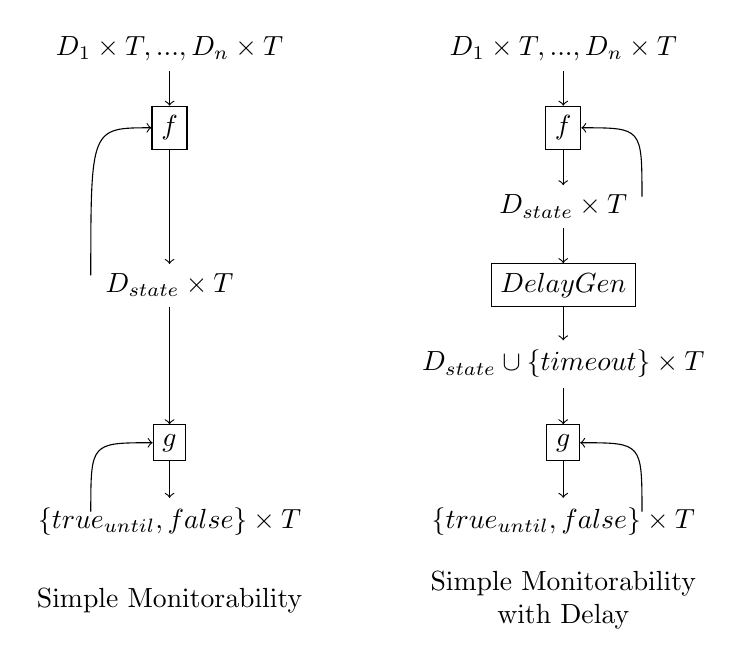
\begin{tikzpicture}
			\node[] (inputRight){$\mathbb{D}_1\times\mathbb{T}, ..., \mathbb{D}_n\times\mathbb{T}$};
			\node[draw, below of=inputRight] (fRight){$f$};
			\node[below of=fRight] (stateRight){$\mathbb{D}_{state}\times\mathbb{T}$};
			\node[draw, below of=stateRight] (delayRight){$DelayGen$};
			\node[below of=delayRight] (stateDelayRight){$\mathbb{D}_{state}\cup\{timeout\}\times\mathbb{T}$};
			\node[draw, below of=stateDelayRight] (gRight){$g$};
			\node[below of=gRight] (outputRight){$\{true_{until}, false\}\times\mathbb{T}$};
			
			\draw[->] (inputRight) -- (fRight);
			
			\node[right of = stateRight] (ha){};
			\node[right of = fRight] (hb){};
			\draw[->] (ha)  .. controls (hb) .. (fRight);
			
			\node[right of = outputRight] (hg){};
			\node[right of = gRight] (hh){};
			\draw[->] (hg)  .. controls (hh) .. (gRight);
			
			\draw[->] (fRight) -- (stateRight);
			\draw[->] (stateRight) -- (delayRight);
			\draw[->] (delayRight) -- (stateDelayRight);
			\draw[->] (stateDelayRight) -- (gRight);
			\draw[->] (gRight) -- (outputRight);
			\node [below of=outputRight, align=center] (h0){Simple Monitorability\\with Delay};
			
			
			\node[left of = inputRight] (h1){};
			\node[left of = h1] (h2){};
			\node[left of = h2] (h3){};
			\node[left of = h3] (h4){};
			
			\node[left of = h4] (inputLeft){$\mathbb{D}_1\times\mathbb{T}, ..., \mathbb{D}_n\times\mathbb{T}$};
			\node[draw, below of=inputLeft] (fLeft){$f$};
			\node[below of = fLeft] (h5){};
			\node[below of=h5] (stateLeft){$\mathbb{D}_{state}\times\mathbb{T}$};
			\node[, below of=stateLeft] (delayLeft){};
			\node[draw, below of=delayLeft] (gLeft){$g$};
			\node[below of=gLeft] (outputLeft){$\{true_{until}, false\}\times\mathbb{T}$};
			\draw[->] (inputLeft) -- (fLeft);
			\draw[->] (fLeft) -- (stateLeft);
			\draw[->] (stateLeft) -- (gLeft);
			\draw[->] (gLeft) -- (outputLeft);
			
			\node[left of = stateLeft] (hc){};
			\node[left of = fLeft] (hd){};
			\draw[->] (hc)  .. controls (hd) .. (fLeft);
			
			\node[left of = outputLeft] (he){};
			\node[left of = gLeft] (hf){};
			\draw[->] (he)  .. controls (hf) .. (gLeft);
			
			\node [below of=outputLeft] {Simple Monitorability};
		\end{tikzpicture}
		\centering
		\caption{Overview Simple Monitorability - with or without \emph{delay}}
		\label{fig:OverviewMonitorability}
	\end{figure}

	\begin{figure}
		\begin{tikzpicture}[state/.style={draw, circle,minimum size=1.5cm, node distance=3cm}]
			\node[state, initial] at (0,0)(qstart)  {$q_{start}$};
			
			\node[state] at(3,2) (qwait1){$q_{wait,d_1}$};
			\node[]at (3,0) (qWaitBla){...};
			\node[state]at(3,-2) (qwaitn){$q_{wait,d_n}$};
			
			\node[state] at(6,0) (qTimeOut){$q_{timeout}$};
			
			\path[->] 	(qstart) edge node[left, near end]{$(d_1, \emptyset, \{c\}, d_1)$} (qwait1)
						(qstart) edge node[left, near end]{$(d_n, \emptyset, \{c\}, d_n)$} (qwaitn)
						(qwait1) edge node[right]{$(\epsilon, \{c > tmr(d_1)\}, \emptyset, timeout)$} (qTimeOut)
						(qwaitn) edge node[right]{$(\epsilon, \{c > tmr(d_n)\}, \emptyset, timeout)$} (qTimeOut)
						(qwait1) edge[loop above] node{$(d_1, \{c \leq tmr(d_1)\}, \{c\}, d_1)$}()
						(qwait1) edge[bend left] node[right, near end]{A}(qwaitn)
						(qwaitn) edge[bend left] node[right, near end]{B}(qwait1)
						(qwaitn) edge[loop below] node{$(d_n, \{c \leq tmr(d_n)\}, \{c\}, d_n)$}()
						(qTimeOut) edge[loop right] node{$\forall d_i \in \mathbb{D}_I:(d_i, \emptyset, \emptyset, timeout)$}();
						
			
		\end{tikzpicture}
		\label{fig:DelayGenerator}
		\caption{Visualization of the Delay Generator. Description A means $(d_n, \{c < tmr(d_1)\}, \{c\}, d_n)$ and description B means $(d_1, \{c < tmr(d_n)\}, \{c\}, d_1)$.}
	\end{figure}
			

			
	\subsection{Not Simple Monitorable}
		Disproving one of the characteristics of \textit{Simple Monitorability} does not necessarily mean, that a property of infinite streams can not be monitored with finite resources. For example, a property, where all parts of \textit{Simple Monitorability} are fulfilled, except the worst case run time of the state transition function, which is dependent on the input streams, but the average run time of this function over every possible trace of this function is not\footnote{In other words, the run time over the entire trace is linear dependent on the length of the trace}. In these cases, a monitor with finite resources can be constructed, which can observe arbitrary long input traces.\\
		If you can prove, that a limitation of the memory consumption, which is required to monitor a property correctly, cannot be given independently of the input streams and their events, it can be safely said, that a property cannot be monitored correctly on arbitrary input traces with finite resources. This is, because the memory of a computation system is always finite. If the required storage space is dependent on the input trace, a set of input streams can always be constructed, which requires an arbitrary large amount of storage space, which is larger than the available memory.

	
		Not all TADL2 constraints are simple monitorable properties, even with delay, because they may require memory resources, which are not independent from the events of the observed trace. Like stated before, correct online monitoring of these constraints is impossible for arbitrary traces, because infinite memory resources may be required. On the other hand, many of these problems are solved by using finite resources, with the hope, that the available resources are enough to cover the inputs of the ''real world''.
		In these cases, a distinction is useful, because the memory or time requirements of some properties grow continuously with every input event, and other constraints only require infinite resources in worst case scenarios. 
		The ones with continuous requirement growth will be called \emph{Always Not Simple Monitorable} and the others \emph{Worst Case Not Simple Monitorable} for the rest of this thesis.\\
		Obviously, the constraints with continuous resource requirement growth cannot be monitored infinitely, but the constraints that only need infinite resources in worst cases can be monitored in many cases.

	 